
%(BEGIN_QUESTION)
% Copyright 2008, Tony R. Kuphaldt, released under the Creative Commons Attribution License (v 1.0)
% This means you may do almost anything with this work of mine, so long as you give me proper credit

In this time-delay relay circuit, the motor will immediately start when the pushbutton is pressed, and continue to run for about 5 seconds after the pushbutton is released.  The green light-emitting diode (LED) is supposed to be on whenever the motor is stopped, and off whenever the motor is running:

$$\includegraphics[width=15.5cm]{i03170x01.eps}$$

However, a problem has developed with this circuit.  Every time the pushbutton switch is pressed, the green LED turns off but the motor never starts.  The LED turns back on after the 5 second delay time.  Based on this information, determine the following:

\vskip 10pt

\begin{itemize}
\item{} \underbar{Two} components or wires in the circuit that you know cannot be failed either open or shorted, besides the 24 volt source.
\vskip 40pt
\item{} \underbar{Two} components or wires in the circuit you think could possibly be bad (either one independently capable of causing the problem), and the type of failure each would be (either open or shorted).
\end{itemize}

\vfil 

\underbar{file i03170}
\eject
%(END_QUESTION)





%(BEGIN_ANSWER)

This is a graded question -- no answers or hints given!

%(END_ANSWER)





%(BEGIN_NOTES)

Clearly, the time-delay feature and the green LED are all working as they should.  This eliminates a majority of the components as possibly being faulted.  The fault must lie somewhere in the circuit where {\it only} the motor would be affected.

\vskip 10pt

\goodbreak
\noindent
{\bf Components known to be in good working condition:}

\begin{itemize}
\item{} Wire from TP1 to TP4
\item{} All wires from TP2 to LED cathode
\item{} $R_1$
\item{} LED
\item{} Pushbutton switch
\end{itemize}

\vskip 10pt

\goodbreak
\noindent
{\bf Components which could possibly be faulted:}

\begin{itemize}
\item{} $R_2$ failed open.
\item{} Motor winding failed open.
\item{} Wire from TP5 to motor failed open.
\item{} Wire from TP7 to motor failed open.
\item{} Lower contact on relay failed open.
\end{itemize}

%INDEX% Troubleshooting review: electric circuits

%(END_NOTES)


